\chapter{Magnetophoresis}\label{ch:magnetophoresis}

%\textit{Magnetophoresis has been proposed to describe the behaviour of a magnetic particle moving through a viscous medium under the influence of an external magnetic field. The appealing feature of the magnetophoresis is that under well-controlled conditions it provides a means for gentle and low-cost particle separation. However, the full control of particle motion in direction and velocity remains complicated, since particle properties and their magnetic response vary quite significantly depending on the manufacturer and its manufacturing processes. This chapter reviews all the basic principles revolving around magnetophoresis.}

\section{Introduction}\label{sec:introductionMagneticParticle}
The increasing interest in single-cell analysis and the rapidly improving sensitivity of molecular biology methods in applications to single-cell genome, transcriptome and signalling analysis put a special emphasis on high quality, high volume, and relatively inexpensive cell separation methods such as those provided by cell magnetophoresis.

Magnetophoresis mainly combines two fields: microfluidic and magnetism. Since fluid dynamics in a microchannel has already been discussed in Chapter~\ref{ch:fluidMechanics}, only the fundamental concepts of magnetism will be briefly recalled here. Further details can be found in one of the many textbooks about magnetism (e.g.~\cite{Morrish2001,Chikazumi1964,Jiles1998}).

% To say why I am doing things
% However, one parameter that has not received any attention is that of the solution viscosity. Here, an investigation was undertaken to study the effect of altering the viscosity of the liquids in the microfluidic chip on the deflection behaviour of particles through the chamber, and also on the separation resolution of two particle populations.

\section{Magnetism}\label{sec:magnetism}
Substances which are magnetized by a magnetic field are called magnetic materials. The term \textit{magnet}, however, is typically used for objects that produce their own persistent magnetic field even in the absence of an applied magnetic field. Only certain classes of materials can actually do this. Most materials, however, produce a magnetic field in response to an applied magnetic field. This phenomenon is generally known as magnetism. There are various kinds of magnetism, and all materials exhibit at least one of them~\cite{Coey2010}.

The magnetism of materials originates from the magnetic moment of electrons in the atom; electron momentum gives rise to magnetic dipole moments. The total magnetic moment of the atom is then given by the vector sum of all its electronic moments~\cite{Cullity2011}. In a bulk magnetic material the net magnetization $\mathbf{M}$ is the vector sum of all the magnetic moments of the atoms per unit volume of the material. However, this does not mean that all the magnetic moments in the entire material will all point in the same direction. Rather what happens is the magnetic pattern is a patchwork of different domains with each domain having its own magnetization vector arising from an alignment of atomic moments within the domain as shown in Figure~\ref{fig:magneticDomain}\cite{Craik1995}. 

\begin{figure}[htb]
\centering
\includegraphics[width=0.5\textwidth]{img/chapters/magneticParticles/magneticDomain_crop.png}
\caption[Magnetic domains in magnetic materials]{Schematic picture of magnetic domains. Arrows represent the direction of the magnetization in the different domains.}%
\label{fig:magneticDomain}%
\end{figure}

Due to this anisotropic alignment of magnetization vectors across different domains, magnetic materials are usually not spontaneously magnetized but exist rather in a demagnetized state, where the overall resultant magnetization vector $\mathbf{M}$ is normally zero. However, by applying an external magnetic field $\mathbf{H}$ these domains can align in the direction of the external field and enhance the overall macroscopic magnetic response in the material. How quickly and with what ease the domains align and whether or not their new alignment remains after the external magnetic field has been removed is material dependent. 

\section{Magnetic field}\label{subsec:magneticField}
A magnetic field is produced whenever there is electrical charge in motion. This can be due to an electrical current flowing in a conductor or produced by a permanent magnet~\cite{Oersted1820,Skomski2008}. In the latter case, the magnetization of a material, as discussed in the previous section (Section~\ref{sec:magnetism}), is expressed in terms of density of net magnetic dipole moments in the material and can be defined as:

\begin{equation}
	\mathbf{M} = \frac{\mathbf{m}}{V}
	\label{eqn:magnetization}
\end{equation}

where $\mathbf{m}$ and $V$ are the total magnetic dipole moment and volume of the material, respectively. The magnetization can also be described by the following linear relation:

\begin{equation}
	\mathbf{M} = \chi \mathbf{H}
	\label{eqn:magnetizationSusceptibility}
\end{equation}

where $\mathbf{H}$ is the applied magnetic field and $\chi$ is the susceptibility of the magnetic material. The magnetic susceptibility of a material describes the ease with which it becomes magnetized in an external magnetic field.

When a magnetic material is placed in a magnetic field, $\mathbf{H}$, the response of the medium is its magnetic induction, also called magnetic flux density. The extent to which a medium responds to the magnetic field depends on the relative permeability of the material. In many media the magnetic flux $\mathbf{B}$ can be assumed to be a linear function of $\mathbf{H}$: %The magnetic flux (this term will be used throughout the remainder of this thesis) can be expressed as: 
\begin{equation}
	\mathbf{B} = \mu_{0}\mu_{r}\mathbf{H}
	\label{eqn:magneticFluxPermeability}
\end{equation}

where $\mu_{0}$ and $\mu_{r}$ are the permeability of free space ($4\pi \times 10^{-7}$ N/A$^{2}$), relative permeability of the material, respectively. 

The relationship between the magnetic flux density $\mathbf{B}$, the magnetization $\mathbf{M}$ and the magnetic field $\mathbf{H}$  is given by:

\begin{equation}
	\mathbf{B} = \mu_{0}(\mathbf{H} + \mathbf{M})
	\label{eqn:magneticFlux}
\end{equation}

If one replaces the magnetization $\mathbf{M}$ (Equation~\ref{eqn:magnetizationSusceptibility}) in Equation~\ref{eqn:magneticFlux} one gets the following expression:

\begin{equation}
	\mathbf{B} = \mu_{0}(1 + \chi)\mathbf{H}
	\label{eqn:magneticFluxSusceptibility}
\end{equation}

%Thus, the relative permeability is related to the susceptibility and the following equation is always true:

%\begin{equation}
%	\mu_{r} = (1 + \chi)
%	\label{eqn:relativePermaeability}
%\end{equation}

%All of this means that a magnetic field $\mathbf{H}$ in amperes per metre gives rise to a magnetic flux density $\mathbf{B}$ measured in Tesla in a medium with a dimensionless relative permeability $\mu_{r}$ or susceptibility $\chi$.
 
\section{Magnetic hysteresis and saturation}\label{sec:hysteresisAndSaturation}
Considering $\chi$ to be a constant in Equation~\ref{eqn:magnetizationSusceptibility}, even though a good approximation at low fields, is an inappropriate assumption for most materials. First, the relationship between $\mathbf{M}$ and $\mathbf{H}$ is generally nonlinear, approaching a finite saturation magnetization $M_{S}$. This represents a condition where magnetic moments within the material are aligned in the direction of the magnetic field $\mathbf{H}$. Second, the magnetization $\mathbf{M}$ is not necessarily a unique function of $\mathbf{H}$. The magnetization curve displays a hysteresis loop, because not all domains might return to their original orientations when $\mathbf{H}$ is decreased after the saturation magnetization value is attained. This phenomenon is illustrated in Figure~\ref{fig:magneticHysteresis}.

% include figuer about hysteresis
\begin{figure}[htb]
\centering
  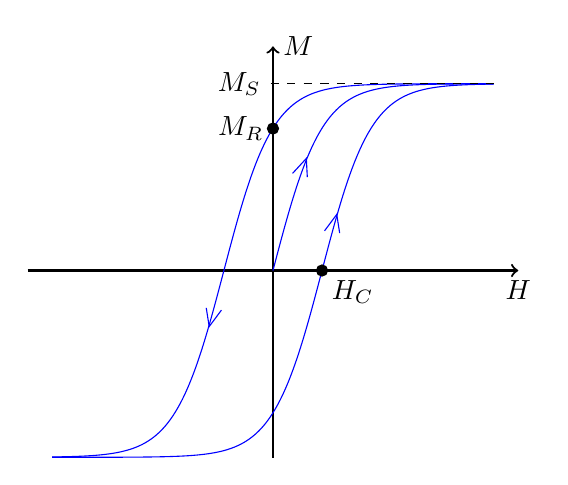
\begin{tikzpicture}
	\begin{axis}[
		xmin=-1.0,xmax=1.2,ymin=0,ymax=1.2,
  		axis lines=none,
  		samples=500]
  		
	 	\draw[thick,->] (axis cs:-1,0.5) -- (axis cs:1,0.5)node[anchor=north] {$H$};
	 	\draw[thick,->] (axis cs:0,-0.1) -- (axis cs:0,1.1)node[anchor=west] {$M$};
		\addplot[blue,domain=-0.9:0.9] {(1)/(1+exp(-10*x+2))};
		\addplot[blue,domain=-0.9:0.9] {(1)/(1+exp(-10*x-2))};									\addplot[blue,domain=0:0.9] {(1)/(1+exp(-10*x))};
		\addplot [only marks,mark=*] coordinates {(0.2,0.5)};
		\addplot [only marks,mark=*] coordinates {(0,0.88)};
		\node[anchor=north west] at (axis cs:0.2,0.5) {$H_{C}$};
	    \node[anchor=east] at (axis cs:0,0.88) {$M_{R}$};
    
    
		\draw[dashed] (axis cs:-0.01,1)node[anchor=east] {$M_{S}$} -- (axis cs:0.9,1);
		\draw[blue] (axis cs:0.08,0.76) -- (axis cs:0.136,0.8) -- (axis cs:0.14,0.75);
		\draw[blue] (axis cs:-0.21,0.394) -- (axis cs:-0.26,0.35) -- (axis cs:-0.272,0.4);
		\draw[blue] (axis cs:0.21,0.606) -- (axis cs:0.26,0.65) -- (axis cs:0.272,0.6);
		
    \end{axis}
  \end{tikzpicture}
\caption[Magnetic hysteresis cycle]{Magnetic hysteresis cycle. The magnetic material will retain a magnetic moment, $M_{R}$, even in the absence of an external field, which essentially creates a new permanent magnet. Only at a coercive field, $H_{C}$, the net magnetic moment of the material will return to zero.}%
\label{fig:magneticHysteresis}%
\end{figure}

Key parameters of the hysteresis loop are the remanent magnetization or remanence $M_{R}$, which is the residual magnetization left in the material after the external field is removed and the coercivity $H_{C}$, which is the magnitude of the field that must be applied in the negative direction to bring the magnetization back to zero. 

%Coercivity and remanence are complemented by parameters describing the loop shape and the area under the loop. In the absence of an external magnetic field, the individual particle dipoles are randomly oriented due to thermal agitation

\section{Magnetic materials and properties}
Magnetic materials encompass a wide variety of materials and their macroscopic magnetic behaviour can be classified into ferro- or ferrimagnetic, paramagnetic and diamagnetic. They are grouped according to their magnetic dipole orientation and bulk magnetic susceptibility. The different kinds of magnetism will be briefly discussed in the following subsections.

\begin{figure}[htb]
        \centering
        \begin{subfigure}[b]{0.28\textwidth}
        \centering
                \includegraphics[width=0.75\textwidth]{img/chapters/magneticParticles/ferromagnetism_crop.png}
                \caption{Ferromagnetism}
                \label{fig:ferromagnetism}
        \end{subfigure}
        %%%%%%%%%%%%%%%%
        \begin{subfigure}[b]{0.28\textwidth}
        \centering
                \includegraphics[width=0.75\textwidth]{img/chapters/magneticParticles/ferrimagnetism_crop.png}
                \caption{Ferrimagnetism}
                \label{fig:ferrimagnetism}
        \end{subfigure}
        %%%%%%%%%%%%%%%%
        \begin{subfigure}[b]{0.28\textwidth}
        \centering
		        \includegraphics[width=0.75\textwidth]{img/chapters/magneticParticles/paramagnetism_crop.png}			
                \caption{Paramagnetism}
                \label{fig:paramagnetism}
        \end{subfigure}
        \caption[Overview and comparison of the magnetic of the different types of magnetism]{Overview and comparison of the different types of magnetism. The magnetic dipole orientation defined the magnetic type.}
        \label{fig:magneticMaterialProperty}
\end{figure}

\subsection{Ferromagnetic and ferrimagnetic materials}\label{subsec:ferromagneticAndFerrimagneticMaterials}
Ferromagnetic and ferrimagnetic materials are the ones normally thought of as magnetic, because these materials are the only ones that can retain a magnetization and become magnets. The magnetic moments interact strongly with an applied magnetic field and their orientation remains stable even after removal of the external field. Thus, ferromagnetic materials exhibit a large and positive magnetic susceptibility ($\chi \gg 0$).

%Different classes of spontaneous magnetization have been identified when there are multiple magnetic moments, whose magnitude and arrangement can be different and arranged anti-parallel. In the case of ferromagnetism, all magnetic moments are aligned parallel to one another, which results in a strong positive interaction between neighbouring moments, whereas in the ferrimagnetic case some magnetic moments are anti-aligned resulting in a weaker net magnetization $\mathbf{M}$, as shown in Figure~\ref{fig:ferromagnetism} and Figure~\ref{fig:ferrimagnetism}~\cite{Neel1948,Chikazumi1964}.

The ease with which the different domains can change their direction differs widely between the different ferro- and ferrimagnetic materials. However, this wide variety of magnetic materials can be rather sharply divided into two groups. If a small applied field suffices to produce saturation, the material is said to be magnetically soft. Other materials, which require a very large field to saturate are called magnetically hard~\cite{Cullity2011,Chikazumi1964}. The difference can be best seen in their hysteresis loops as depicted in Figure~\ref{fig:magneticSoftMagneticHard}.

\begin{figure}[htb]
        \centering
        \begin{subfigure}[b]{0.48\textwidth}
                \begin{tikzpicture}[scale=1.0]
                \begin{axis}[
		  		axis lines=none,
  				samples=500]
  		
			 		\draw[thick,->] (axis cs:-0.8,0.5) -- (axis cs:0.8,0.5)node[anchor=north east] {$H$};
		 			\draw[thick,->] (axis cs:0,-0.1) -- (axis cs:0,1.1)node[anchor=north east] {$M$};
					\addplot[blue,domain=-0.7:0.7] {(1)/(1+exp(-30*x+1))};
					\addplot[blue,domain=-0.7:0.7] {(1)/(1+exp(-30*x-1))};
					\addplot[blue,domain=0:0.7] {(1)/(1+exp(-30*x))};
					
					\draw[blue] (axis cs: -0.066,0.42) -- (axis cs: -0.049,0.39) -- (axis cs: -0.026,0.42);
					\draw[blue] (axis cs: 0.066,0.58) -- (axis cs: 0.049,0.61) -- (axis cs: 0.026,0.58);
					\draw[blue] (axis cs: 0.015,0.713) -- (axis cs: 0.035,0.75) -- (axis cs: 0.045,0.71);
			    \end{axis}
            	
				\end{tikzpicture}
                \caption{Soft magnetic}
                \label{fig:magneticSoft}
        \end{subfigure}
        %%%%%%%%%%%%%%%%
        \begin{subfigure}[b]{0.48\textwidth}
                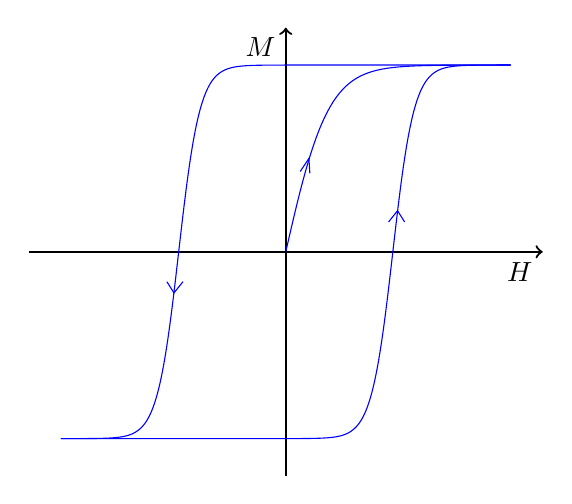
\begin{tikzpicture}[scale=1.0]
                \begin{axis}[
		  		axis lines=none,
		  		samples=500]
  		
	 				\draw[thick,->] (axis cs:-0.8,0.5) -- (axis cs:0.8,0.5)node[anchor=north east] {$H$};
				 	\draw[thick,->] (axis cs:0,-0.1) -- (axis cs:0,1.1)node[anchor=north east] {$M$};
					\addplot[blue,domain=-0.7:0.7] {(1)/(1+exp(-30*x+10))};
					\addplot[blue,domain=-0.7:0.7] {(1)/(1+exp(-30*x-10))};
					\addplot[blue,domain=0:0.7] {(1)/(1+exp(-15*x))};
					
					\draw[blue] (axis cs: 0.045,0.715) -- (axis cs: 0.072,0.75) -- (axis cs: 0.075,0.71);
					\draw[blue] (axis cs: 0.32,0.58) -- (axis cs: 0.348,0.61) -- (axis cs: 0.37,0.58);
					\draw[blue] (axis cs: -0.32,0.42) -- (axis cs: -0.348,0.39) -- (axis cs: -0.37,0.42);
					
				\end{axis}
				
				\end{tikzpicture}
                \caption{Hard magnetic}
                \label{fig:magneticHard}
        \end{subfigure}
        \caption[Hysteresis loops for soft and hard magnetic materials]{Hysteresis loop for observed in the $M-H$ curve for ferromagnetic material. a.) shows a soft magnetic behaviour and b.) a hard magnetic behaviour.}
        \label{fig:magneticSoftMagneticHard}
\end{figure}

\subsection{Paramagnetic materials}\label{subsec:paramagneticMaterials}
Like ferromagnetic species, paramagnetic materials contain magnetic moments which align when exposed to a magnetic field such that they form a weak net magnetic moment, which means their magnetic susceptibility is small and positive ($\chi > 0$). 

However, unlike ferromagnetic materials, they do not exhibit magnetic remanence upon removal of the field as the individual magnetic moments become randomized due to thermal agitation and do not interact with each other. Thus, paramagnetic materials are only magnetized in the presence of an externally applied field, and once the field is removed the magnetization is lost~\cite{Chikazumi1964,Coey2010}.

\subsection{Superparamagnetic materials}\label{subsec:superparamagneticMaterials}
Even if its name suggests a subtype of paramagnetism, superparamagnetism is actually a special form of magnetism with characteristics from both ferromagnetism and paramagnetism. When the length scale of the magnetic material becomes smaller than a critical size ($10-20$ nm), the ferro- or paramagnetic grains can essentially be considered as individual magnetic domains and their magnetization is a single magnetic moment~\cite{Ohandley2000}. At this scale, the available thermal energy becomes of the same order as the magnetic energy, causing the magnetic moment to immediately align randomly in space, after the magnetic field has been removed. Therefore, the coercivity and remanence is substantially equal to zero and thus, no hysteresis can be observed~\cite{Brown1963,McNab1968,Rosensweig2013}. 
 
This behaviour can be described by the N\'{e}el relaxation time which describes the time needed for a magnetic moment to change its orientation~\cite{Neel1949}:

\begin{equation}
	\tau = \tau_{0}\cdot \text{exp}\big(\frac{\Lambda V}{k_{B}T}\big)
	\label{eqn:neelRelaxationTime}
\end{equation}

where $\Lambda V$ is the height of the energy barrier and $k_{B}T$ the thermal energy. The different parameters $\Lambda$, $V$, $k_{B}$ and $T$ are the magnetic anisotropy energy density, grain volume, Boltzmann constant and the temperature, respectively. $\tau_{0}$ is the material characteristic time scale, normally in the order of $10^{-9}-10^{-10}$ seconds.

%%%%%%%%
Since the crystalline anisotropy energy is proportional to the volume of the nanoparticle, there exists a critical size below which the particles cannot retain its~\cite{14} preferred magnetization orientation inside the material's crystalline structure. 

In the last few decades, there have been significant advances in synthesizing fluidic suspensions of magnetorheological fluids, typically composed of a spherical polymer matrix which encapsulates a dispersion of magnetic nanoparticle grains. If the magnetic grains are small enough and spaced sufficiently far apart inside the polymer matrix, then the composite particle will behave superparamagnetically yet it will have a large dipole moment due to the collective response of the large number of magnetic grains inside the bead. The magnetic susceptibility of these commercially available beads is typically in the range of $0.1-1.0$. 

%%%%%%%%

\subsection{Diamagnetic materials}\label{subsec:dieamagneticMaterials}
Diamagnetism materials exhibit a net magnetization which is opposite to the direction of the externally applied magnetic field and thus, are repelled by the applied magnetic field. That means, diamagnetic materials have a small negative magnetic susceptibility ($-1<\chi<0$)~\cite{Cullity2011,Jiles1998}. 

The opposed magnetic moment of diamagnetic substances is generally a very weak effect and loses its opposing magnetization after removal of the applied magnetic field. 

\section{Forces on a magnetic microparticle}
A magnetic particle that is in suspension in a liquid and is being exposed to a magnetic field, experiences a set of forces. However, the magnetic force and the Stokes drag force are the most dominant forces. Other forces such as, gravity, buoyancy and also Saffman forces can be neglected for microscopic particles because of their small size ($<2$ $\mu m$)~\cite{McCloskey2000,Wirix-Speetjens2005,Saffman1965}. 

\subsection{Magnetic force on a magnetized object}
The external magnetic field will magnetize the particle, inducing a magnetic moment $m_{p}$ in the direction of the field. Thus, the magnetic force on a point-like magnetic dipole can be given as:

\begin{equation}
	\mathbf{F}_{m} = (\mathbf{m}_{p} \cdot \nabla)\mathbf{B}
	\label{eqn:magneticForceMagneticMoment}
\end{equation}

with $\mathbf{m}_{p}$ the net magnetic moment of the particle and $\nabla |\mathbf{B}|$ the gradient of the magnetic flux density. By assuming a constant magnetic field across the volume of the particle one can substitute the expression for the magnetic moment by using Equation~\ref{eqn:magnetization} and Equation~\ref{eqn:magnetizationSusceptibility}. This leads to the following equation:

\begin{equation}
	\mathbf{F}_{m} = V_{p} \chi_{p}(\mathbf{H}\cdot \nabla)\mathbf{B} 
	\label{eqn:magneticForceMagneticField}
\end{equation} 

where $V_{p}$ and $\chi_{p}$ are the volume and the effective susceptibility of the particle, respectively. Alternatively, the magnetic force on a particle (Equation~\ref{eqn:magneticForceMagneticField}) can also be expressed with respect to the magnetic flux density $\mathbf{B}$:

\begin{equation}
	\mathbf{F}_{m} = \frac{V_{p} \chi_{p}}{\mu_{0}}\Bigl( \mathbf{B}\cdot \nabla \Bigr)\mathbf{B} 
	\label{eqn:magneticForceMagneticFlux}
\end{equation} 

Equation~\ref{eqn:magneticForceMagneticFlux} is most commonly used in the literature and will also be used throughout this thesis. If the particle is suspended in a viscous fluid Equation~\ref{eqn:magneticForceMagneticFlux} needs to be slightly modified since the susceptibility of the surrounding medium should be to be taken into account:

\begin{equation}
	\mathbf{F}_{m} = \Delta \chi V_{p} \left(\frac{\nabla |\mathbf{B}|^{2}}{2\mu_{0}}\right)
	\label{eqn:magneticForceFluid}
\end{equation}

where $\Delta \chi = \chi_{p}-\chi_{f}$ describes the difference in relative magnetic susceptibility between the magnetic particle ($\chi_{p}$) and the surrounding medium ($\chi_{f}$).

It is important to note here, that Equation~\ref{eqn:magneticForceMagneticFlux} assumes the magnetic media to be linearly polarizable, for which the magnetic susceptiblity $\chi_{p}$ is independent of the applied magnetic field. In general, this is a valid assumption for all materials in a sufficiently weak field. 

\subsection{Drag force on a spherical microparticle}
In the case of micrometre sized spherical particles at low Reynolds number, Stokes regime is found to be applicable (see Section~\ref{sec:particleLadenFlowInMicrofluidicSystems}). The drag force, opposing the magnetic force induced migration, on a particle of radius $r_{p}$ travelling at relative velocity $\Delta u = u_{f}-u_{p}$, between the particle and the fluid, in a medium of viscosity $\eta_{f}$, can be written as:

\begin{equation}
	F_{D} = 6\pi\eta_{f} r_{p} \Delta u
	\label{eqn:dragForceOnParticle}
\end{equation}

%The overall relative magnetic susceptibility of the composite is further influenced by the demagnetization effect, which is related to the self-generated magnetic field in the space surrounding the particle. In consequence, the effective relative magnetic susceptibility $\chi_{eff}$ for spherical magnetic microparticle can be expressed as:

%\begin{equation}
%	\chi_{eff} = \frac{3\chi_{m}}{3+\chi_{m}}
%\end{equation}

%where $\chi_{m}$ is the material susceptibility of the enclosed magnetic nanoparticles. 

\section{Theory of magnetophoresis}\label{sec:theoryOfMagnetophoresis}
Using the two described dominant forces, magnetic force ($\mathbf{F}_{m}$) and Stokes drag ($\mathbf{F}_{d}$), Newton's second law of motion can then be written as:

\begin{equation}
	\frac{\partial \mathbf{u}_{p}}{\partial t} = \mathbf{F}_{m}+\mathbf{F}_{d}
	\label{eqn:equationOfMotion}
\end{equation}

For micro-sized particles, a terminal velocity is reached in a matter of microseconds (see Appendix~\ref{sec:terminalVelocity}), in which case it is appropriate to assume:

\begin{equation}
	\mathbf{F}_{m} = -\mathbf{F}_{d}
	\label{eqn:equationOfMotionSimplified}
\end{equation}

From this simplified equation of motion (Equation~\ref{eqn:equationOfMotionSimplified}) one obtains the magnetically induced terminal velocity of the particle:

\begin{equation}
	\mathbf{u}_{p} = \frac{\Delta\chi_{p} V_{p}}{6\pi\eta r_{p}} \cdot \left(\frac{\nabla |\mathbf{B}|^{2}}{2\mu_{0}}\right)
	\label{eqn:terminalVelocity}
\end{equation}

An interesting interpretation of the expression given in Equation~\ref{eqn:terminalVelocity}, is that it depends on a purely particle related term and a field related term; it is a product of particle and suspending viscous medium properties and the applied magnetic field properties. 

The two factors of this product can be usefully defined as the magnetophoretic mobility of the particle $\nu_{p}$ and the magnetophoretic driving force $S$, given by:

\begin{eqnarray}
		\nu_{p} &=& \frac{\Delta \chi V_{p}}{6\pi\eta r_{p}} \label{eqn:magnetophoreticMobility} \\ \nonumber \\
		S &=& \frac{\nabla |\mathbf{B}|^{2}}{2\mu_{0}}
		\label{eqn:magnetophoreticDrivingForce}
\end{eqnarray}

\section{Magnetophoretic mobility}\label{sec:magnetophoreticMobility}
The magnetophoretic mobility $\nu_{p}$ is the characteristic property of the magnetic particle that quantifies how it moves in a non-homogeneous magnetic field and is a parameter that determines the performance of magnetic separation devices. Therefore, knowing this particle property is absolutely crucial in order to accurately predict the particles' trajectories.

The magnetophoretic mobility, which can be usefully compared to electrophoretic mobility, is the magnetically induced velocity, $u_{p}$, divided by the magnetic energy gradient, $S$, and can be mathematically represented by:

\begin{equation}
	\nu_{p} = \frac{u_{p}}{S} = \frac{u_{p}}{\left(\frac{\nabla |\mathbf{B}|^{2}}{2\mu_{0}}\right)} 
	\label{eqn:magneticMobility}
\end{equation}

To study the magnetophoretic mobility, the magnetically induced velocity, given in Equation~\ref{eqn:terminalVelocity}, has been measured for different types of particles as well as for different particle agglomeration configurations.
The study will help to evaluate the \textit{magnetic responsiveness} of single particles and agglomerates which is essential when designing magnetic separation systems.

%Continuous methods have been described [299] however, these methods meet certain difficulties. The agglomeration of MPs is a particular problem. The greater the number of MPs within close proximity of each other, the greater the magnetic force acting upon them. Under high concentration scenarios, particle agglomeration is unavoidable [33, 34]. An understanding of the magnetic properties of particle agglomerates is required to allow for predictability when designing a continuous flow system. 

\subsection{Magnetophoretic mobility of superparamagnetic particles}\label{subsec:magnetophoreticMobilityOfSuperparamagneticParticles}
Due to the increasing interest in magnetic particles, different low cost and easily functionalizable microparticles are now commercially available from various manufacturers. Depending on their fabrication process, the different magnetic particles have slightly different magnetic composition, and thus differ in their magnetophoretic mobility. 

In this section, the magnetophoretic mobility of five types of magnetic microparticles from two different manufacturers (Table~\ref{tab:particleType}) is investigated using a microscope setup. The particles' multi-phase structure, described in Section~\ref{sec:superparamagneticMicroparticles}, as well as their superparamagnetic properties has been verified by Fonnum \etal~\cite{Fonnum2005} for the Dynabeads particles and confirmed by Chemicell GmBH for their particles~\cite{chemicellConversation}.

\begin{table}[htb]
\begin{center}
\caption[Physical characteristics of the five tested particle types]{Physical characteristics of the five tested types of particles as stated by the manufacturers~\cite{chemicellConversation,dynabeads2015}}\vspace{1ex}
\label{tab:particleType}
\begin{tabular}{llccc}\hline
Particle type 			& Manufacturer 	& Diameter  	& Iron content 	& Density   \\ 
						& 				& [$\mu$m] 		& [wt. $\%$]	& [g/cm$^3$] \\
\hline
ScreenMAG-Silanol 		& Chemicell 	& 1.0 			& 40 			& 2.25  \\
SiMAG-Silanol 			& Chemicell 	& 1.0 			& 40 			& 2.25 \\
MyOne 					& Dynabeads 	& 1.05 			& 26 			& 1.7 \\
M280 					& Dynabeads 	& 2.8 			& 12 			& 1.4 \\
M270 					& Dynabeads 	& 2.8 			& 14 			& 1.6 \\ \hline
\end{tabular}
\end{center}
\end{table}

To compare the mobility of different single microparticles, their drift velocities in stationary fluid (deionized water) was observed, similar to the work of H\"{a}feli \etal~\cite{Haefeli2013}. In Ref~\cite{Haefeli2013} the particles were kept at a constant distance from the magnet; in this work, however, their velocity was optically measured at different distance away from the magnet using an inverted microscope (Leitz Wetzlar, Germany) with a long working distance $20\times$ objective lens (Comar Optics, Cambridge, UK) and a CCD camera ($\mu$Eye Imaging Development Software, Germany) attached. The trajectories of single particles moving towards the magnet were observed in a Fast Read 102 microscope counting slide which consists of a set of easy-to-fill fluid \textit{observation chambers}. Each observation chamber has a depth of 100 $\mu$m and a counting grid etched to its surface. The counting grid has a dimensions $5 \times 2$ mm and helped determining the viewing location, as depicted in Figure~\ref{fig:magnetophoreticMobilityExperimentSchematic}.

\begin{figure}[htb]%
\centering
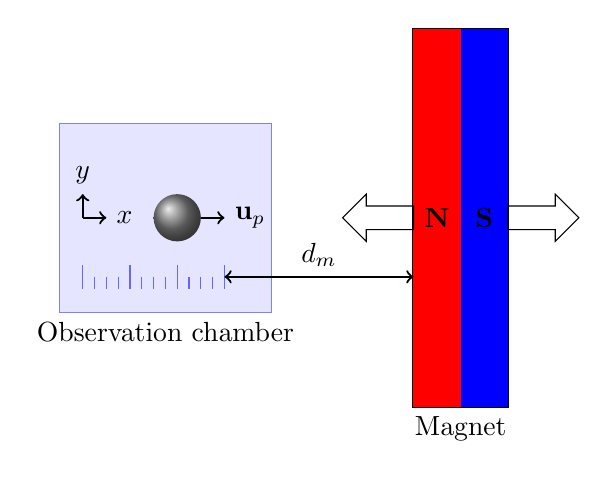
\begin{tikzpicture}[scale=0.6]
	\filldraw[color=blue!50!, fill=blue!10] (-2.5,-2) rectangle (2,2);
	\node[anchor=north] at (-0.25,-2) {Observation chamber};
	
	\draw[->,thick] (-2,0) -- (-1.5,0)node[anchor=west]{$x$};
	\draw[->,thick] (-2,0) -- (-2,0.5)node[anchor=south]{$y$};
	
	\draw[color=blue!60!](-2,-1.5) -- (-2,-1); 
	\draw[color=blue!60!](-1.75,-1.5) -- (-1.75,-1.25); 
	\draw[color=blue!60!](-1.5,-1.5) -- (-1.5,-1.25); 
	\draw[color=blue!60!](-1.25,-1.5) -- (-1.25,-1.25); 
	\draw[color=blue!60!](-1,-1.5) -- (-1,-1); 
	\draw[color=blue!60!](-0.75,-1.5) -- (-0.75,-1.25); 
	\draw[color=blue!60!](-0.5,-1.5) -- (-0.5,-1.25); 
	\draw[color=blue!60!](-0.25,-1.5) -- (-0.25,-1.25); 
	\draw[color=blue!60!](0,-1.5) -- (0,-1); 
	\draw[color=blue!60!](0.25,-1.5) -- (0.25,-1.25); 
	\draw[color=blue!60!](0.5,-1.5) -- (0.5,-1.25); 
	\draw[color=blue!60!](0.75,-1.5) -- (0.75,-1.25); 
	\draw[color=blue!60!](1,-1.5) -- (1,-1); 
	
  	\shade[ball color=gray] (0,0) circle (0.5);
  	\draw[->,thick] (0.5,0) -- (1.0,0) node[anchor=west] {$\mathbf{u}_{p}$};

  	\draw[thick](5,-4) rectangle (7,4);
  	
  	\fill[red] (5,-4) rectangle (6,4)node[black,font=\bf,pos=.5]{N};
  	\fill[blue] (6,-4) rectangle (7,4)node[black,font=\bf,pos=.5]{S};
	\node[anchor=north] at (6,-4) {Magnet};
	
	\draw(7,0.25) -- (8,0.25) -- (8,0.5) -- (8.5,0) -- (8,-0.5) -- (8,-0.25) -- (7,-0.25) -- cycle;
	\draw(5,0.25) -- (4,0.25) -- (4,0.5) -- (3.5,0) -- (4,-0.5) -- (4,-0.25) -- (5,-0.25) -- cycle;
	
  	\draw[<->,thick] (1,-1.25) -- node[anchor=south]{$d_{m}$} (5,-1.25);
\end{tikzpicture}
\caption[Schematic of experimentally used particle velocity tracking setup]{Schematic drawing showing the experimental setup used to determine the magnetically induced velocity of magnetic particles. The distance $d_{m}$ is varied step wise from $10$ mm to $16$ mm with a step size of $2$ mm. Figure shown here is not drawn to scale.}
\label{fig:magnetophoreticMobilityExperimentSchematic}%
\end{figure}

Prior to the measurement all particles had been diluted to a solution of $0.9-1.4\times 10^{5}$ particles/ml. The concentrations were then confirmed by observing the number of particles on the counting grid of the observation chamber. Visual inspection of previous experiments had shown that such low concentrations successfully avoid particle interaction. The particle solution was then put in an ultrasonic bath for at least five minutes to break up all possible aggregates and also agitated to fully suspend the particles. A volume of $20$ $\mu$l of each microparticle solution was pipetted into an observation chamber. The liquid solution is drawn into the channel via capillary action. Once the particle solution had filled the observation chamber and the particles had become stationary, an external magnetic field was applied by accurately position a N42 neodymium (NdFeB) magnet ($42\times8\times10$ mm) adjacent to the FastRead counting slide. The magnet dimensions are much larger than the observation chamber. Thus, a uniform magnetic field along the width of the observation chamber can be assumed and edge effects can safely be neglected. The permanent magnet is attached to a translation stage, which allowed accurate movement of the magnet to different positions, $d_{m}$, away from the counting grid (see Figure~\ref{fig:magnetophoreticMobilityExperimentSchematic}).
% The permanent magnet is attached to a high precision transverse translation stage, which allowed accurate movement of the magnet to different positions, $d_{m}$, away from the counting grid (see Figure~\ref{fig:magnetophoreticMobilityExperimentSchematic}). 

The particle trajectories of single magnetic particles for the magnet being positioned at $10$, $12$, $14$ and $16$ mm away from the counting grid were recorded and analysed offline using the freely available software \textit{ImageJ} with the open source particle tracking plug-in \textit{MTrackJ}. The magnification of the microscope enables the individual particles and multiple particle complexes to be clearly distinguished. Particles were tracked moving in the $x$ direction towards the magnet over a distance of $55$ $\mu$m, which is equivalent to one traverse of the field of view of the microscope camera. The magnetically induced velocity of single particles has been measured for each of the five types of particles and for all four magnet positions. Particles travelling with an atypical velocity were discarded in the measurement, to avoid including data from particles that are clearly interacting with the chamber surface. Also particle agglomerations have been ignored from this analysis. 

Figure~\ref{fig:magnetophoreticDriftVelocityAtDifferentPositions} shows the drift velocities of the five particle types at different distances, $d_{m}$, from the magnet surface.

\begin{figure}[htb]
   \centering
   \includegraphics[width=0.75\textwidth]{img/chapters/magneticParticles/magnetophoreticDriftVelocityAtDifferentPositionsErrorBars3.eps}
   \caption[Magnetically induced velocities of different particle types]{Magnetically induced velocities of each of the five particle types measured at four different distances $d_{m}$ from the magnet face.}
   \label{fig:magnetophoreticDriftVelocityAtDifferentPositions}
\end{figure}

The magnitude of the magnetophoretic mobility, $\nu_{p}$, was calculated according to Equation~\ref{eqn:magneticMobility}. The magnetophoretic driving force at the various positions of the magnet is estimated by using the software package ANSYS Maxwell. The simulated flux density dropped from $65$ mT to $30$ mT when the distance $d_{m}$ is increased from $10$ mm to $16$ mm, and the corresponding flux gradient was found to change from $10$ mT/mm to $3.6$ mT/mm. The magnetic flux density, $\mathbf{B}$, was also measured using a Hall effect probe (5100 Series Sypris) to verify the numerical simulation. The simulation showed a maximum discrepancy of $12\%$ compared to the Hall measurements; which, due to the size of the probe and positioning tolerance, is within an acceptable measurement error (see Chapter~\ref{ch:numericalMethods}). The magnetic mobilities of each of the particle types have been determined for the distinct magnet positions and are depicted in Figure~\ref{fig:magnetophoreticMobilityAtDifferentPositions}.

\begin{figure}[htb]
   \centering
   \includegraphics[width=0.75\textwidth]{img/chapters/magneticParticles/magnetophoreticMobilityAtDifferentPositionsErrorBars3.eps}
   \caption[Magnetophoretic mobility of different particle types]{Magnetophoretic mobility of each of the five particle types measured at four different distances $d_{m}$ from the magnet face.}
   \label{fig:magnetophoreticMobilityAtDifferentPositions}
\end{figure}

Despite the fact that the drift velocity in Figure~\ref{fig:magnetophoreticDriftVelocityAtDifferentPositions} shows an increase as the magnetic microparticles approach the magnet, their mobility in Figure~\ref{fig:magnetophoreticMobilityAtDifferentPositions} appears to be less sensitive to distance $d_{m}$ from the magnet and one can assume that the particles do not reach their magnetic saturation. Figure~\ref{img:magnetophoreticMobilityDistribution} shows a typical histogram of the measured mobilities for the SiMAG Chemicell particles. Although the histogram has a clearly defined peak, it also shows a large variance in magnetic mobility.

\begin{figure}[htb]
   \centering
   \includegraphics[width=0.75\textwidth]{img/chapters/magneticParticles/magnetophoreticMobilityDistribution.eps}
   \caption[Histogram of magnetophoretic mobility of $1$ $\mu$m sized Chemicell SiMAG particles]{Histogram of the magnetophoretic mobility of Chemicell SiMAG $1 \mu$m superparamagnetic particle in deionized water. The mode of the distribution is estimated at $0.0585$ $\text{mm}^{3}/\text{T}\cdot\text{A}\cdot\text{s}$.}
   \label{img:magnetophoreticMobilityDistribution}
\end{figure}

The averaged magnetophoretic mobilities for each of the five particle types is used to derive the magnetic susceptibility, tabulated in Table~\ref{tab:particleMobility}.

\begin{table}[htb]
\begin{center}
\caption[Experimentally found magnetophoretic mobility and susceptibility of superparamagnetic particles using magnetophoresis]{The experimentally found mean magnetophoretic mobility obtained for the five types of superparamagnetic microparticles using magnetophoresis. Experiments were performed in deionized water over a magnetic field range of $30$ mT to $65$ mT.}\vspace{1ex}
\label{tab:particleMobility}
\begin{tabular}{lccr}\hline
Particle type 		& $\nu_{p}$ & $\chi_{p}$  & \multicolumn{1}{l}{Number of} \\ 
					& [mm$^3$/T$\cdot$A$\cdot$s] & & \multicolumn{1}{l}{particles analysed} \\ \hline
ScreenMAG-Silanol 	& $0.017\pm 0.007$ & $0.30$ & 246 \\
SiMAG-Silanol 		& $0.059\pm 0.042$ & $1.06$ & 557 \\
MyOne 	 			& $0.020\pm 0.010$ & $0.31$ & 51 \\
M280 				& $0.054\pm 0.015$ & $0.12$ & 267 \\
M270 				& $0.079\pm 0.023$ & $0.18$ & 103 \\ \hline
\end{tabular}
\end{center}
\end{table}

\subsection{Magnetophoretic mobiltiy of superparamagnetic agglomerates}\label{subsec:magnetophoreticMobiltiyOfSuperparamagneticAgglomerates}
As soon as superparamagnetic microparticles are exposed to an external magnetic field they become magnetized, which causes them to form particle chains if they are in close proximity to each other. This chain formation could be seen during the magnetophoretic mobility study of single particles described in the previous section (Section~\ref{sec:superparamagneticMicroparticles}). These particle agglomerations have a different magnetophoretic mobility compared to single particles due to their increased magnetic force and change in Stokes' drag. The change in mobility also has an effect on the magnetic separation process and thus needs to be treated differently in magnetic separation simulations. 

The self-assembled chains align in the same direction as the magnetic field lines, but drift in the direction of increasing magnetic energy density, i.e. towards the magnet. Magnetic field lines and magnetic energy density gradient do not necessarily point in the same direction, as illustrated in Figure~\ref{fig:particleAgglomeratesTravellingTowardsMagnet}.

\begin{figure}[htb]
        \centering
        \begin{subfigure}[b]{0.45\textwidth}
        \begin{center}
                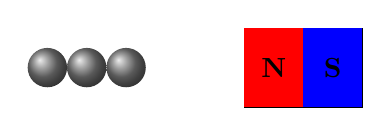
\begin{tikzpicture}[scale=0.5]
                
				 \shade[ball color=gray] (-1,0) circle (0.5);
				 \shade[ball color=gray] (0,0) circle (0.5);
				 \shade[ball color=gray] (1,0) circle (0.5);
  
			  	 \draw (4,-1) rectangle (7,1);
				 \fill[red] (4,-1) rectangle (5.5,1)node[black,font=\bf,pos=.5]{N};
			  	 \fill[blue] (5.5,-1) rectangle (7,1)node[black,font=\bf,pos=.5]{S};				
				
				\end{tikzpicture}
                \caption{Parallel alignment}
        \end{center}
        \end{subfigure}
        %%%%%%%%%%%%%%%%
        \begin{subfigure}[b]{0.45\textwidth}
        \begin{center}
                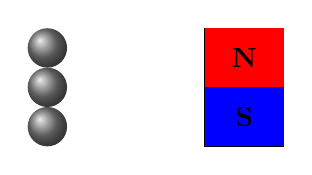
\begin{tikzpicture}[scale=0.5]
                
                \shade[ball color=gray] (0,-1) circle (0.5);
				 \shade[ball color=gray] (0,0) circle (0.5);
				 \shade[ball color=gray] (0,1) circle (0.5);
				 
                \draw (4,-1.5) rectangle (6,1.5);
				 \fill[red] (4,0) rectangle (6,1.5)node[black,font=\bf,pos=.5]{N};
			  	 \fill[blue] (4,-1.5) rectangle (6,0)node[black,font=\bf,pos=.5]{S};		
				
                
				\end{tikzpicture}
                \caption{Perpendicular alignment}
        \end{center}
        \end{subfigure}
        \caption[Schematic of magnetic particle agglomerates travelling towards a permanent magnet]{A schematic of magnetic particle agglomerates travelling towards a permanent magnet. In configuration a) the magnetic field lines are parallel to the direction of the magnetically induced velocity. In configuration b) the field lines and travelling velocity are perpendicular to each other. Figure is not in scale.}
        \label{fig:particleAgglomeratesTravellingTowardsMagnet}
\end{figure}

The hydrodynamic drag force on a chain depends on its length and orientation. Unfortunately, the hydrodynamic resistance of elongated bodies is more complicated to determine than for a simple sphere. No exact solution has been reported in the microfluidic literature to the author's knowledge and therefore approximate methods have been employed for elongated bodies. Since the hydrodynamic drag mainly depends on the body aspect ratio or, in this case, the number of particles, the chain of particles moving in axial or lateral direction in low Reynolds number flow can be adapted as a longitudinal elliptic body, with a circular cross-section equal to the diameter of the spherical particles, $r_{p}$, and the long axis equal to the length of the number of particles in the chain, $n \times 2r_{p}$. Using this approximation the hydrodynamic resistance acting on a chain of particles moving in parallel or orthogonal to its long axis can be approximated as follows~\cite{Happel2012,Kasper1985}:

\begin{align}
	F_{\|} &= 4\pi\eta_{f} r_{p} u \Biggl[ \frac{n^{2}-1}{\left(\frac{2n^{2}-1}{\sqrt{n^{2}-1}}\right) \cdot \ln \left( n + \sqrt{n^{2}-1}\right)-n} \Biggr] \label{eqn:parallel}\\
	F_{\bot} &= 8\pi\eta_{f} r_{p} u \Biggl[ \frac{n^{2}-1}{\left(\frac{2n^{2}-3}{\sqrt{n^{2}-1}}\right)\cdot \ln \left( n + \sqrt{n^{2}-1}\right)+n} \Biggr] \label{eqn:perpendicular}
\end{align}

where $F_{\|}$ and $F_{\bot}$ describe the drag force of the chain when its long axis is aligned or orthogonal to its moving direction, respectively. The parameter $n$ is the number of beads in the chain, $\eta_{f}$ the dynamic viscosity of the fluid, $r_{p}$ diameter of a single bead in the chain and $u$ the velocity with which the chain moves. Note that the two equations above (Equation~\ref{eqn:parallel} and Equation~\ref{eqn:perpendicular}) only apply for $n \geq 2$.

By using Equation~\ref{eqn:parallel} or Equation~\ref{eqn:perpendicular} in the proposed magnetophoresis model one can determine the magnetophoretic mobility of a chain with different particle length. In a first approximation, one can assume that the total magnetic moment of a chain is given by the summation of all magnetic moments of the particles in a chain. In other words, dipole interaction between neighbouring particles has been assumed to be negligible compared to changes in the drag force.

In order to explore the effect of Stokes' drag upon the mobility of chains of microparticles and to demonstrate the models proposed, two magnetic orientation configurations were investigated experimentally. Videos of particles that had formed chains were recorded and their magnetically induced velocity was measured. The particle concentration has been increased ($1.8\times 10^{7}$ particles/ml) compared to the measurements of individual particles in order to increase the number of agglomeration examples. 

To compare the mobility of chains of different length with the model described above it is sufficient to only consider a normalized terminal velocity. The normalized velocity is obtained by dividing the chain velocity by the magnetic drift velocity of a single bead. Due to this normalization the different particle types, given in Table~\ref{tab:particleType}, can be directly compared to each other. 

Figure~\ref{fig:magnetophoreticVelocityOfDifferentChainLenghts} shows the experimental data compared to the model for both magnet orientations, and confirms that the longitudinal elliptical body approximation is a sufficiently accurate predictor of the drift velocity for chains of different particle lengths. 

\begin{figure}[htb]
        \centering
        \begin{subfigure}[b]{0.48\textwidth}
                \includegraphics[width = \textwidth]{img/chapters/magneticParticles/terminalVelocityRatioParticleChainParallel.eps}
                \caption{Parallel alignment}
        \end{subfigure}
        \hfill
        \begin{subfigure}[b]{0.48\textwidth}
                \includegraphics[width = \textwidth]{img/chapters/magneticParticles/terminalVelocityRatioParticleChainPerpendicular.eps}
                \caption{Perpendicular alignment}
        \end{subfigure}
        \caption[Normalized magnetophoretically induced velocity of different particle chain lengths]{The normalized ratio of the magnetophoretically induced velocity per chain of magnetic particles to the magnetophoretically induced velocity of a single magnetic particle travelling towards a magnet a) parallel and b) perpendicular to the field lines. The dotted curves represent the data calculated from the proposed model.}
        \label{fig:magnetophoreticVelocityOfDifferentChainLenghts}
\end{figure}

\section{Particle magnetization measurement}
In order to obtain independent and consistent magnetic information for all particles types given in Table~\ref{tab:particleType}, their magnetization curve was measured using a superconducting quantum interference device (SQUID). The SQUID has become a widely used instrument for determining moment of magnetization as a function of an externally applied magnetic field and is also used for studying the magnetic properties of superparamagnetic particles such as the magnetic susceptibility and saturation magnetization~\cite{Cullity2011}. The SQUID relaxometry technique and the apparatus used for the measurements reported have been described in details in other literature~\cite{Cullity2011,Flynn2005,Adolphi2009}. Thus, only a brief explanation is given here. The SQUID sensor measures the magnetic moment by magnetizing the sample using an applied magnetic field pulse ranging from $-5$ T to $5$ T in amplitude and with a frequency of $0.5-4$ Hz.

A sample of the different magnetic particle types ($1-30$ mg) was dried in an oven at $65^\circ$ C. The dry particles were placed in a sample holder where no rotation was possible. The sample holder was sealed to ensure a fixed particle position and attached to a SQUID probe. The probe is lowered into the SQUID measurement system (Quantum Design Magnetic Property Measurement System MPMS-XL) where a magnetic field of $\pm5$ Tesla was applied at a temperature of $300$ K. 

Figure~\ref{fig:histeresisLoopParticleManufacturer} shows the hysteresis loops for the different particle types. From these curves the saturation magnetization, $M_{S}$ was estimated and the magnetic susceptibility of the particles, $\chi_{p}$, was obtained by taking the ratio of the sample magnetization and the applied magnetic field at four different magnetic fields over the range of $30-65$ mT, corresponding to the magnetic flux density of the mobility measurement for single particles. Figure~\ref{fig:histeresisLoopParticleManufacturer} shows that all samples start saturating at a magnetic flux density of $0.1$ T. The difference in saturation magnetization for each type comes from the different iron oxide content.
 

\begin{figure}[htb]
        \centering
        \begin{subfigure}[b]{0.48\textwidth}
                \includegraphics[width = \textwidth]{img/chapters/magneticParticles/hysteresisLoopChemicellAndInset.PNG}
                \caption{Chemicell}
                \label{fig:hysteresisLoopChemicell}
        \end{subfigure}
        \hfill
        \begin{subfigure}[b]{0.48\textwidth}
                \includegraphics[width = \textwidth]{img/chapters/magneticParticles/hysteresisLoopDynabeadsAndInset.PNG}
                \caption{Dynabeads}
                \label{fig:hysteresisLoopDynabeads}
        \end{subfigure}
        \caption[Magnetization curves of Chemicell and Dynabeads particles]{Magnetization curves of the different particle types within an applied magnetic field range of $\pm1$ T. Inset figures show a close up in the field range of $\pm40$ mT. (a) Magnetization curves of Chemicell particles. (b) Magnetization curves of Dynabeads particles. The curves were measured with a Quantum Design MPMS-XL SQUID magnetometer at room temperature ($300$ K).}
\label{fig:histeresisLoopParticleManufacturer}
\end{figure}

The hysteresis loops in Figure~\ref{fig:histeresisLoopParticleManufacturer} directly give the magnetization of each of the five types of particles at a specific applied magnetic field (Figure~\ref{fig:hysteresisLoopChemicell} for Chemicell particles and Figure~\ref{fig:hysteresisLoopDynabeads} for Dynabeads particles) and incorporate all magnetic properties (e.g. remanence) of the particle sample. The  remanence was observed to be no more than $1.5$ mT; refer to Shevkoplyas \etal~\cite{Shevkoplyas2007}.

Using the measured hysteresis loops the susceptibilities were determined at the four values of magnetic field corresponding to the data reported in Section~\ref{subsec:magnetophoreticMobilityOfSuperparamagneticParticles} . From these four values the mean was calculated for comparison with the average susceptibility values reported in Table~\ref{tab:particleMobility}.

The mean susceptibility values and the saturation magnetization found here, compare well with what has been stated in the literature~\cite{Haefeli2005,Wise2015,Fonnum2005,Zborowski2002}. Additionally, it shows that the magnetophoretic mobility measurement is a promising technique to determine the susceptibility of magnetic particles. 
 
The magnetic susceptibility and the saturation magnetization obtained from the SQUID data are summarized in Table~\ref{tab:particleSusceptibility}.

\begin{table}[htb]
\begin{center}
\caption[Experimentally found magnetophoretic mobility and susceptibility of superparamagnetic particles using SQUID]{SQUID results for the magnetic susceptibility of the magnetic particles .}\vspace{1ex}
\label{tab:particleSusceptibility}
\begin{tabular}{lcr}\hline
Particle type:  	&  $\chi_{p}$  				& $M_{S}$ [emu/g]  \\ 
 					& ($|\mathbf{B}|< 65$ mT) 	& ($|\mathbf{B}|\geq 1$ T)\\ \hline
ScreenMAG-Silanol 	& $0.53 \pm 0.12$ 						& 19.2 \\
SiMAG-Silanol 		& $1.20 \pm 0.21$ 						& 34.7 \\
MyOne 				& $0.26 \pm 0.05$ 						& 10.1 \\
M280 				& $0.19 \pm 0.04$ 						& 7.4 \\
M270 				& $0.18 \pm 0.04$ 						& 6.9 \\ \hline
\end{tabular}
\end{center}
\end{table}

The insets in Figure~\ref{fig:histeresisLoopParticleManufacturer} reveal that assuming a linear relationship between magnetization and applied field is only a simplified model, even at weak magnetic fields. The observed monotonic increase in magnetophoretic mobility with increasing distance from the magnet (Figure~\ref{fig:magnetophoreticMobilityAtDifferentPositions}) is not accounted for in a simplified model and in some circumstances should be taken into consideration.

Table~\ref{tab:proportionalSusceptibilityMobilityIncrease} compares the reduction in magnetophoretic mobility for each particle type as they approach the permanent magnet from a distance of $d_{m} = 16$ mm to $d_{m} = 10$ mm.  The ratio of mobility at these two distances is obtained from the particle tracking experiment for each particle type.  This ratio is compared to the ratio of susceptibility obtained from the SQUID hysteresis loops at the magnetic field values simulated at the same distances. It is apparent that the change in relative mobility is consistent with the relative change in susceptibility; confirming the conclusion that particle tracking of magnetic particles is a promising technique for determination of drift mobility and susceptibility.

\begin{table}[htb]
\begin{center}
\caption[Proportional change in magnetophoretic mobility and susceptibility]{Proportional increase of the measured magnetophoretic mobility and susceptibility at $d_{m}=10$ mm and $d_{m}=16$ mm.}\vspace{1ex}
\label{tab:proportionalSusceptibilityMobilityIncrease}
\begin{tabular}{lccccc}\hline
Ratio:  				& ScreenMAG & SiMAG  & MyOne & M280 & M270  \\ 
\hline
$\nu_{d_{m}=10}/\nu_{d_{m}=16}$ 		& 62.5 & 64.0 & 61.4 & 68.5 & 68.2 \\
$\chi_{d_{m}=10}/\chi_{d_{m}=16}$ 	& 64.5 & 65.8 & 64.9 & 61.9 & 62.4 \\
\hline
\end{tabular}
\end{center}
\end{table}

\section{Conclusion}\label{sec:conclusionMagneticParticles}
In this chapter the theoretical framework behind the manipulation of magnetic microparticles was discussed and the magnetic properties of the magnetic particles that will be used in the trajectory model were investigated. A simple particle tracking method has been developed that allows the analysis of the magnetically induced drift velocity of magnetic particles in a known magnetic field gradient. The trajectories of the magnetic particles within the magnetic field as single particles as well as particle complexes were observed. Based on the observed drift velocity one can determine the overall magnetic responsiveness, magnetophoretic mobility, of the particles. 

In the case of single particles, Dynabeads' M270 showed the greatest magnetophoretic mobility followed by Chemicell's SiMAG particles, the Dynabeads' type M280 and MyOne, in a descending order. ScreenMAG, exhibits the smallest magnetophoretic mobility. This differences in mobility can be explained by the different iron content and hydrodynamic radius of the particle types. The large discrepancy between the two Chemicell types might be a consequence of their different host matrix.

The mobility is measured over a range of $30-65$ mT using a permanent magnet and remain almost constant compared to the variation in magnetic drift velocity. Estimates of the susceptibility compared to those obtained by SQUID measurement suggest that particle tracking is a promising technique for determination of susceptibility of magnetic particles over a range of magnetic flux density.

However, the hysteresis curves obtained from the SQUID measurements have shown the practical limits of the model assuming that $\chi_{p}$ is constant and remanence is zero.  The monotonic reduction in mobility of the beads as they approach the permanent magnet can be linked to a change in susceptibility with magnetic field strengths. Thus, a magnetic flux density of $30-60$ mT cannot be assumed as weak and the nonlinear behaviour of susceptibility should be taken into consideration.

For the case of particle agglomerates, where the field gradient was kept the same, chains of magnetic particles aligned with the field lines travelled more quickly towards the magnet than an equally long chain which was aligned perpendicular. The experimental results match the proposed model for both magnet orientations and can therefore be used as a good approximation to scale the magnetophoretic mobility of particle agglomerates. 

This section highlights the differences in physical properties of the many commercially available magnetic particles and make it evident that some particle types are potentially more suitable for LOC magnetic separation than others. Since the separation time is often a limiting factor, especially for continuous magnetic separation, but also for test tube separation, particles with a higher magnetophoretic mobility are preferred. 

The magnetophoretic mobilities and susceptibility values found here will help scientist to predict the motion of magnetic particles more accurately.

%The mobility measurements as well as the SQUID measurements have shown 
%
%The motion of magnetic microparticles that are under the influence of a magnetic field gradient have been investigated.  
%
%There is a good agreement for the susceptibility between the two different measurements methods. 
%
%A method has been developed that allows the analysis of the magnetically induced drift velocity of MPs in a known magnetic gradient. The trajectories of the MPs within a magnetic field, as single particles, chains and complexes, were observed. The Dynabead M270 had the greatest magnetophoretic mobility. Chains of MPs aligned with the field lines of the magnet.
%
%This study shows that the magnetic drift velocity of MPs formed into chains or attached to NBs can be predicted using simple approximations to the increase in drag forces.  Tracking the movement of MPs attached to a biomarker will enable the quantification, and a method to separate, successfully captured biomarkers. The measurement of magnetophoretic mobility may be an effective tool for the detection of captured bacteria by the MP if the attachment is of comparable size. 
%
%
%We have investigated the motion of magnetic microparticles that are under the influence of a magnetic field gradient in a microfluidic channel through experiments and numerical simulations. There is good agreement between both measurements and simulations. Two dimensionless global parameters П1 and П2 are able to characterize the capture efficiency (Φ), which in a steady flow of a homogeneous suspension of magnetic microspheres represents the ratio of the number of particles captured in the device to the number of particles entering the channel. For various combinations of the operating parameters applied to a specified geometry, the capture efficiency depends solely on П1 that characterizes the ratio of the magnetic and viscous drag forces on the particles. If the geometry is altered, the values of Φ in various channels depend on П2, which is the ratio of the distance of the magnet from the channel to the channel height. These correlations provide a method to rationally design magnetic particle separators over a wide range of operating conditions.

%%%%%%%%%%%%%%%%%%%%%%%%%%%%%%%%%%%%%%%%%%%%%%%%%%%%%%%%
%\section{Text}
%The past decade has seen an unprecedented increase in interest for utilizing magnetic beads in microfluidic devices (pamme). Magnetic beads can be seamlessly integrated into systems on a chip due to, their micro/nano size, large specific surface areas available for binding biomolecules, being independent of reagent chemistry or photo-bleaching as well as being biocompatible with no toxicity index. Superparamagnetic type magnetic beads have attracted a lot of attention in recent times. They do have magnetic moment in the absence of an external magnetic field but become magnetized once an external magnetic field is applied. Hence, unlike ferromagnetic materials, they do not exhibit a remanent magnetization. This not only prevent the agglomoration of magnetic beads but also enables an externaml magnetic field to control the beads remotely. Hence, magnetic beads are for example used in a variety of in vivo biomedical applications such as targeted drug delivery, where it is possible to transport drugs or medicine to a specific region in the body. 
%%[http://ac.els-cdn.com/S0167931710005563/1-s2.0-S0167931710005563-main.pdf?_tid=d996bbfc-ee52-11e4-9997-00000aacb362&acdnat=1430300213_edc44d9200bc59e9a3032fc98ba3ff87]
%
%The magnetic properties of individual single superparamagnetic beads, such as their magnetic susceptibility, field dependence and saturation magnetization are the crucial parameters in the performance of magnetic based bioassays, since the the magnetic characteristics of individual bio-functionalized beads dominate the sensor's behavior and efficiency. 
%
%Additionally, since the materials in the particles are ferro- or ferrimagnetic, the magnetic susceptibility is very high and so the attraction towards the field is very strong. However, when the field is removed, thermal energy is again able to affect the moments of the particles, returning them to their original state whereby they exhibit no time-averaged net magnetic moment. As a result, the particles lose their magnetization and are able to disperse back into the media they are present in.
%
%The in essence ferro- or paramagnetic grains within the particle are generally so small, so that these can be considered to be individual magnetic domains. Every grain has a preferred state of magnetization along its easyaxis, but its magnetization can easily flip because of thermal fluctuations. The time between two flips is called the Neel relaxation time. Due to the high number of grains in the particle with independently and fast flipping magnetizations, the net magnetic moment of the particle is zero in the absence of an applied magnetic field. However, if an external magnetic field is applied, the grains within the superparamagnetic particle preferably magnetize along the direction of the applied magnetic field. A net magnetic moment is created, similar to the mechanism in paramagnetism. The magnetic susceptibility of a superparamagnetic material is however much higher~\cite{Ohandley2000}.
%
%When the length scale of the material becomes small, however, the number of domains decreases until there is a single domain when the characteristic size of the material is below some critical size ($10-20$ nm). The remanence of a single magnetic domain is found to be zero and therefore no hysteresis loop can be seen. The magnetic moment of such single domains is regarded to move freely. Thus, the remanent state could be taken as that in which the moment orientations are randomly distrbuted in space. This magnetic behavior is known as superparamagnetic.
